\documentclass[10pt,a4paper]{article}
\usepackage[margin=20mm,top=17mm,bottom=17mm]{geometry}
\usepackage{fontspec}
\setmainfont{texgyretermes}[Extension=.otf,UprightFont=*-regular,BoldFont=*-bold,
  ItalicFont=*-italic,BoldItalicFont=*-bolditalic]
\setsansfont{texgyreheros}[Extension=.otf,UprightFont=*-regular,BoldFont=*-bold,
  ItalicFont=*-italic,BoldItalicFont=*-bolditalic,Scale=0.94]
\setmonofont{texgyrecursor}[Extension=.otf,UprightFont=*-regular,BoldFont=*-bold,
  ItalicFont=*-italic,BoldItalicFont=*-bolditalic,Scale=0.90]
\usepackage{booktabs}
\usepackage{longtable}
\usepackage{array}
\usepackage{graphicx}
\usepackage{fancyvrb}
\usepackage{fvextra}
\usepackage{amsmath,amssymb}
\usepackage{caption}
\captionsetup{font=small,labelfont=bf,justification=justified,singlelinecheck=false}
\usepackage{titlesec}
\titleformat{\section}{\normalfont\large\bfseries}{}{0pt}{}
\titleformat{\subsection}{\normalfont\normalsize\bfseries}{}{0pt}{}
\titleformat{\subsubsection}{\normalfont\normalsize\itshape}{}{0pt}{}
\titlespacing*{\section}{0pt}{11pt plus 2pt minus 1pt}{4pt}
\titlespacing*{\subsection}{0pt}{9pt plus 2pt minus 1pt}{3pt}
\titlespacing*{\subsubsection}{0pt}{7pt plus 1pt}{2pt}
\usepackage{enumitem}
\setlist[itemize]{leftmargin=1.2em,topsep=2pt,itemsep=1pt,parsep=0pt}
\setlist[enumerate]{leftmargin=1.4em,topsep=2pt,itemsep=1pt,parsep=0pt}
\usepackage[hidelinks]{hyperref}
\usepackage{microtype}
\setlength{\parindent}{0pt}
\setlength{\parskip}{3.2pt plus 1pt}
\setlength{\emergencystretch}{2.5em}
\renewcommand{\arraystretch}{1.04}
\begin{document}
\begin{center}
{\Large\bfseries Appendix A -\allowbreak{} full result tables\par}
\vspace{3pt}

\end{center}
\vspace{-2pt}
Every table below is generated from \texttt{results/\allowbreak{}raw/\allowbreak{}} by \texttt{python -\allowbreak{}m tsfdi report-\allowbreak{}figures}; the report body quotes the compact forms and points here for the per-\allowbreak{}site and per-\allowbreak{}magnitude detail.

\section*{A.1 Detection by attack family and magnitude (all cells)}
{\small
\setlength{\tabcolsep}{2pt}
\setlength{\LTleft}{\fill}
\setlength{\LTright}{\fill}
\begin{longtable}{lrrrrrrrrrrr}
\toprule
var. & family & $\sigma$ & n & det. rate & miss rate & delay med. & q1 & q3 & AUPRC & units & gain \\
\midrule
\endfirsthead
\toprule
var. & family & $\sigma$ & n & det. rate & miss rate & delay med. & q1 & q3 & AUPRC & units & gain \\
\midrule
\endhead
\bottomrule
\endlastfoot
PRCP & noise\_\allowbreak{}shaped & 0.5 & 60 & 0.55 & 0.45 & 39 & 13 & 95 & 0.048 & 0.247 & nan \\
PRCP & noise\_\allowbreak{}shaped & 1 & 60 & 0.583 & 0.417 & 37 & 13.5 & 95 & 0.061 & 0.495 & nan \\
PRCP & noise\_\allowbreak{}shaped & 1.5 & 60 & 0.717 & 0.283 & 34 & 12 & 90 & 0.069 & 0.742 & nan \\
PRCP & noise\_\allowbreak{}shaped & 2 & 60 & 0.767 & 0.233 & 23.5 & 11.5 & 79 & 0.082 & 0.99 & nan \\
PRCP & noise\_\allowbreak{}shaped & 3 & 60 & 0.817 & 0.183 & 19 & 11 & 70 & 0.137 & 1.563 & nan \\
PRCP & ramp & 0.5 & 60 & 0.633 & 0.367 & 75.5 & 24.75 & 112 & 0.076 & 0.215 & nan \\
PRCP & ramp & 1 & 60 & 0.633 & 0.367 & 81 & 28.5 & 102.5 & 0.08 & 0.426 & nan \\
PRCP & ramp & 1.5 & 60 & 0.7 & 0.3 & 67 & 28 & 98 & 0.138 & 0.616 & nan \\
PRCP & ramp & 2 & 60 & 0.8 & 0.2 & 74.5 & 28 & 99 & 0.237 & 0.787 & nan \\
PRCP & ramp & 3 & 60 & 0.85 & 0.15 & 61 & 29 & 96.5 & 0.269 & 1.124 & nan \\
PRCP & scaling & 0.5 & 60 & 0.683 & 0.317 & 39 & 14 & 102 & 0.062 & 0.804 & 0.545 \\
PRCP & scaling & 1 & 60 & 0.75 & 0.25 & 25 & 9 & 73 & 0.117 & 1.702 & 1.249 \\
PRCP & scaling & 1.5 & 60 & 0.833 & 0.167 & 17 & 9.25 & 54.5 & 0.218 & 2.696 & 2.111 \\
PRCP & scaling & 2 & 60 & 0.883 & 0.117 & 16 & 8 & 54 & 0.338 & 3.815 & 3.132 \\
PRCP & scaling & 3 & 60 & 0.9 & 0.1 & 13 & 6 & 44 & 0.394 & 6.407 & 5.647 \\
PRCP & step & 0.5 & 60 & 0.467 & 0.533 & 60.5 & 13 & 95 & 0.059 & 0.317 & nan \\
PRCP & step & 1 & 60 & 0.617 & 0.383 & 52 & 14 & 84 & 0.067 & 0.601 & nan \\
PRCP & step & 1.5 & 60 & 0.767 & 0.233 & 51 & 12 & 80.75 & 0.213 & 0.847 & nan \\
PRCP & step & 2 & 60 & 0.8 & 0.2 & 24 & 10.25 & 59 & 0.277 & 1.062 & nan \\
PRCP & step & 3 & 60 & 0.867 & 0.133 & 18 & 6.75 & 48.5 & 0.368 & 1.548 & nan \\
TMAX & noise\_\allowbreak{}shaped & 0.5 & 160 & 0.538 & 0.462 & 47.5 & 20.25 & 82.5 & 0.041 & 0.452 & nan \\
TMAX & noise\_\allowbreak{}shaped & 1 & 160 & 0.744 & 0.256 & 28 & 16 & 62 & 0.051 & 0.904 & nan \\
TMAX & noise\_\allowbreak{}shaped & 1.5 & 160 & 0.925 & 0.075 & 21.5 & 12.75 & 40 & 0.131 & 1.356 & nan \\
TMAX & noise\_\allowbreak{}shaped & 2 & 160 & 0.956 & 0.044 & 15 & 9 & 28 & 0.244 & 1.808 & nan \\
TMAX & noise\_\allowbreak{}shaped & 3 & 160 & 1 & 0 & 11 & 5 & 16.25 & 0.454 & 2.712 & nan \\
TMAX & ramp & 0.5 & 160 & 0.644 & 0.356 & 64 & 27.5 & 115.5 & 0.053 & 0.59 & nan \\
TMAX & ramp & 1 & 160 & 0.794 & 0.206 & 65 & 39 & 103 & 0.068 & 1.179 & nan \\
TMAX & ramp & 1.5 & 160 & 0.894 & 0.106 & 65 & 40 & 91.5 & 0.203 & 1.769 & nan \\
TMAX & ramp & 2 & 160 & 0.956 & 0.044 & 58 & 39 & 81 & 0.309 & 2.359 & nan \\
TMAX & ramp & 3 & 160 & 0.994 & 0.006 & 48 & 31.5 & 66.5 & 0.344 & 3.538 & nan \\
TMAX & scaling & 0.5 & 160 & 0.612 & 0.387 & 28 & 14 & 63 & 0.048 & 0.59 & 0.045 \\
TMAX & scaling & 1 & 160 & 0.806 & 0.194 & 20 & 10 & 51 & 0.163 & 1.179 & 0.089 \\
TMAX & scaling & 1.5 & 160 & 0.95 & 0.05 & 13 & 5 & 29.5 & 0.498 & 1.769 & 0.134 \\
TMAX & scaling & 2 & 160 & 0.994 & 0.006 & 10 & 4 & 21 & 0.54 & 2.359 & 0.179 \\
TMAX & scaling & 3 & 160 & 0.988 & 0.012 & 5 & 2 & 12.75 & 0.539 & 3.538 & 0.268 \\
TMAX & step & 0.5 & 160 & 0.606 & 0.394 & 33 & 16 & 71 & 0.045 & 0.59 & nan \\
TMAX & step & 1 & 160 & 0.788 & 0.212 & 24.5 & 13 & 62.25 & 0.132 & 1.179 & nan \\
TMAX & step & 1.5 & 160 & 0.9 & 0.1 & 13 & 7 & 32 & 0.469 & 1.769 & nan \\
TMAX & step & 2 & 160 & 0.981 & 0.019 & 11 & 5 & 20 & 0.527 & 2.359 & nan \\
TMAX & step & 3 & 160 & 0.988 & 0.012 & 5 & 2.25 & 11 & 0.539 & 3.538 & nan \\
TMIN & noise\_\allowbreak{}shaped & 0.5 & 60 & 0.433 & 0.567 & 32 & 19.75 & 69.75 & 0.042 & 0.629 & nan \\
TMIN & noise\_\allowbreak{}shaped & 1 & 60 & 0.683 & 0.317 & 28 & 14 & 77 & 0.059 & 1.258 & nan \\
TMIN & noise\_\allowbreak{}shaped & 1.5 & 60 & 0.917 & 0.083 & 18 & 10 & 52.5 & 0.145 & 1.886 & nan \\
TMIN & noise\_\allowbreak{}shaped & 2 & 60 & 0.983 & 0.017 & 13 & 8 & 30.5 & 0.336 & 2.515 & nan \\
TMIN & noise\_\allowbreak{}shaped & 3 & 60 & 1 & 0 & 9 & 5 & 14 & 0.594 & 3.773 & nan \\
TMIN & ramp & 0.5 & 60 & 0.517 & 0.483 & 77 & 37.5 & 101 & 0.052 & 0.744 & nan \\
TMIN & ramp & 1 & 60 & 0.767 & 0.233 & 82 & 49 & 104 & 0.088 & 1.488 & nan \\
TMIN & ramp & 1.5 & 60 & 0.933 & 0.067 & 76.5 & 49 & 94.25 & 0.254 & 2.232 & nan \\
TMIN & ramp & 2 & 60 & 0.967 & 0.033 & 67.5 & 49 & 82.5 & 0.329 & 2.976 & nan \\
TMIN & ramp & 3 & 60 & 1 & 0 & 53.5 & 46 & 63.25 & 0.343 & 4.464 & nan \\
TMIN & scaling & 0.5 & 60 & 0.533 & 0.467 & 35.5 & 18 & 77 & 0.045 & 0.744 & 0.126 \\
TMIN & scaling & 1 & 60 & 0.967 & 0.033 & 26.5 & 12 & 66 & 0.303 & 1.488 & 0.253 \\
TMIN & scaling & 1.5 & 60 & 0.967 & 0.033 & 13 & 4 & 32.75 & 0.538 & 2.232 & 0.379 \\
TMIN & scaling & 2 & 60 & 1 & 0 & 8 & 1.75 & 30 & 0.573 & 2.976 & 0.506 \\
TMIN & scaling & 3 & 60 & 1 & 0 & 4 & 0 & 16 & 0.607 & 4.464 & 0.758 \\
TMIN & step & 0.5 & 60 & 0.483 & 0.517 & 46 & 29 & 76 & 0.042 & 0.744 & nan \\
TMIN & step & 1 & 60 & 0.883 & 0.117 & 39 & 27 & 70 & 0.143 & 1.488 & nan \\
TMIN & step & 1.5 & 60 & 0.967 & 0.033 & 22 & 13 & 36.5 & 0.487 & 2.232 & nan \\
TMIN & step & 2 & 60 & 1 & 0 & 15.5 & 8.75 & 22.25 & 0.519 & 2.976 & nan \\
TMIN & step & 3 & 60 & 1 & 0 & 6 & 2 & 10.25 & 0.515 & 4.464 & nan \\
\end{longtable}
}

\section*{A.2 Replay detection by window length}
{\small
\setlength{\tabcolsep}{3pt}
\setlength{\LTleft}{\fill}
\setlength{\LTright}{\fill}
\begin{longtable}{lrrrrrrrr}
\toprule
var. & length & n & det. rate & miss rate & delay med. & q1 & q3 & AUPRC \\
\midrule
\endfirsthead
\toprule
var. & length & n & det. rate & miss rate & delay med. & q1 & q3 & AUPRC \\
\midrule
\endhead
\bottomrule
\endlastfoot
PRCP & 3 & 60 & 0.267 & 0.733 & 9.5 & 2 & 19.25 & 0.002 \\
PRCP & 5 & 60 & 0.4 & 0.6 & 4.5 & 3 & 12.5 & 0.004 \\
PRCP & 7 & 60 & 0.433 & 0.567 & 5 & 3 & 10.75 & 0.007 \\
PRCP & 14 & 60 & 0.75 & 0.25 & 9 & 5 & 13 & 0.017 \\
PRCP & 21 & 60 & 0.783 & 0.217 & 9 & 5.5 & 13 & 0.032 \\
TMAX & 3 & 160 & 0.675 & 0.325 & 1 & 0 & 2 & 0.028 \\
TMAX & 5 & 160 & 0.712 & 0.288 & 1 & 0 & 3 & 0.146 \\
TMAX & 7 & 160 & 0.888 & 0.112 & 2 & 0 & 6 & 0.166 \\
TMAX & 14 & 160 & 0.962 & 0.037 & 2 & 0 & 6 & 0.194 \\
TMAX & 21 & 160 & 0.975 & 0.025 & 2 & 0 & 6 & 0.233 \\
TMIN & 3 & 60 & 0.467 & 0.533 & 1 & 0 & 2 & 0.005 \\
TMIN & 5 & 60 & 0.583 & 0.417 & 2 & 0 & 4 & 0.014 \\
TMIN & 7 & 60 & 0.767 & 0.233 & 3 & 0 & 6 & 0.091 \\
TMIN & 14 & 60 & 0.833 & 0.167 & 3 & 0 & 6 & 0.15 \\
TMIN & 21 & 60 & 0.917 & 0.083 & 4 & 0.5 & 6 & 0.167 \\
\end{longtable}
}

\section*{A.3 False alarms per (site, variable) on clean data}
{\footnotesize
\setlength{\tabcolsep}{3pt}
\setlength{\LTleft}{\fill}
\setlength{\LTright}{\fill}
\begin{longtable}{>{\raggedright\arraybackslash}p{0.229\linewidth}rrrrrr>{\raggedright\arraybackslash}p{0.083\linewidth}r>{\raggedright\arraybackslash}p{0.118\linewidth}}
\toprule
site & var. & years & events & alarms/\allowbreak{}yr & in extreme & extreme d & calib. rate & target & over \\
\midrule
\endfirsthead
\toprule
site & var. & years & events & alarms/\allowbreak{}yr & in extreme & extreme d & calib. rate & target & over \\
\midrule
\endhead
\bottomrule
\endlastfoot
CARTHAGE & TMAX & 5.002 & 8 & 1.599 & 0 & 80 & 2 & 1 & 0.599 \\
CARTHAGE & TMIN & 5.002 & 3 & 0.6 & 0 & 27 & 1 & 1 & -\allowbreak{}0.4 \\
CARTHAGE & PRCP & 5.002 & 4 & 0.8 & 0 & 16 & 4 & 1 & -\allowbreak{}0.2 \\
JENDOUBA & TMAX & 5.002 & 12 & 2.399 & 1 & 92 & 0 & 1 & 1.399 \\
JENDOUBA & TMIN & 5.002 & 18 & 3.599 & 0 & 34 & 2 & 1 & 2.599 \\
JENDOUBA & PRCP & 5.002 & 16 & 3.199 & 0 & 14 & 4 & 1 & 2.199 \\
GAFSA & TMAX & 5.002 & 16 & 3.199 & 3 & 100 & 3 & 1 & 2.199 \\
GAFSA & TMIN & 5.002 & 2 & 0.4 & 0 & 50 & 2 & 1 & -\allowbreak{}0.6 \\
GAFSA & PRCP & 5.002 & 31 & 6.197 & 0 & 16 & 3 & 1 & 5.197 \\
MERSA\_\allowbreak{}MATRUH & TMAX & 5.002 & 19 & 3.798 & 1 & 92 & 5 & 1 & 2.798 \\
MERSA\_\allowbreak{}MATRUH & TMIN & 5.002 & 7 & 1.399 & 0 & 45 & 1 & 1 & 0.399 \\
KHARGA & TMAX & 5.002 & 31 & 6.197 & 1 & 46 & 3 & 1 & 5.197 \\
KHARGA & TMIN & 5.002 & 27 & 5.398 & 0 & 63 & 1 & 1 & 4.398 \\
NAVACERRADA & TMAX & 5.002 & 7 & 1.399 & 0 & 73 & 1 & 1 & 0.399 \\
NAVACERRADA & TMIN & 5.002 & 5 & 1 & 0 & 46 & 1 & 1 & -\allowbreak{}0 \\
NAVACERRADA & PRCP & 5.002 & 7 & 1.399 & 1 & 22 & 1 & 1 & 0.399 \\
MONT\_\allowbreak{}AIGOUAL & TMAX & 5.002 & 5 & 1 & 0 & 88 & 5 & 1 & -\allowbreak{}0 \\
MONT\_\allowbreak{}AIGOUAL & TMIN & 5.002 & 24 & 4.798 & 0 & 42 & 6 & 1 & 3.798 \\
MONT\_\allowbreak{}AIGOUAL & PRCP & 5.002 & 8 & 1.599 & 1 & 10 & 0 & 1 & 0.599 \\
FELDBERG & TMAX & 5.002 & 4 & 0.8 & 0 & 55 & 2 & 1 & -\allowbreak{}0.2 \\
FELDBERG & TMIN & 5.002 & 10 & 1.999 & 0 & 52 & 2 & 1 & 0.999 \\
FELDBERG & PRCP & 5.002 & 6 & 1.2 & 0 & 15 & 0 & 1 & 0.2 \\
CABAUW & TMAX & 5.002 & 4 & 0.8 & 0 & 60 & 0 & 1 & -\allowbreak{}0.2 \\
CABAUW & TMIN & 5.002 & 14 & 2.799 & 2 & 46 & 2 & 1 & 1.799 \\
CABAUW & PRCP & 5.002 & 8 & 1.599 & 0 & 18 & 1 & 1 & 0.599 \\
HELSINKI\_\allowbreak{}KAISANIEMI & TMAX & 5.002 & 14 & 2.799 & 0 & 84 & 3 & 1 & 1.799 \\
HELSINKI\_\allowbreak{}KAISANIEMI & TMIN & 5.002 & 8 & 1.599 & 1 & 70 & 3 & 1 & 0.599 \\
HELSINKI\_\allowbreak{}KAISANIEMI & PRCP & 5.002 & 4 & 0.8 & 0 & 21 & 0 & 1 & -\allowbreak{}0.2 \\
ALTA\_\allowbreak{}LUFTHAVN & TMAX & 5.002 & 3 & 0.6 & 0 & 77 & 0 & 1 & -\allowbreak{}0.4 \\
ALTA\_\allowbreak{}LUFTHAVN & TMIN & 5.002 & 7 & 1.399 & 0 & 58 & 2 & 1 & 0.399 \\
ALTA\_\allowbreak{}LUFTHAVN & PRCP & 5.002 & 9 & 1.799 & 0 & 15 & 1 & 1 & 0.799 \\
MIAMI\_\allowbreak{}INTL & TMAX & 5.002 & 19 & 3.798 & 1 & 55 & 7 & 1 & 2.798 \\
MIAMI\_\allowbreak{}INTL & TMIN & 5.002 & 13 & 2.599 & 0 & 48 & 4 & 1 & 1.599 \\
MIAMI\_\allowbreak{}INTL & PRCP & 5.002 & 14 & 2.799 & 1 & 21 & 1 & 1 & 1.799 \\
\end{longtable}
}

\section*{A.4 Diagnosis confidence calibration}
{\small
\setlength{\tabcolsep}{4.5pt}
\setlength{\LTleft}{\fill}
\setlength{\LTright}{\fill}
\begin{longtable}{lrrrr}
\toprule
band & n & conf. & acc. & gap \\
\midrule
\endfirsthead
\toprule
band & n & conf. & acc. & gap \\
\midrule
\endhead
\bottomrule
\endlastfoot
high & 73 & 0.833 & 0.959 & -\allowbreak{}0.126 \\
low & 88 & 0.543 & 0.25 & 0.293 \\
medium & 73 & 0.686 & 0.575 & 0.111 \\
\end{longtable}
}

\section*{A.5 Efficiency: latency and memory per station}
{\small
\setlength{\tabcolsep}{3pt}
\setlength{\LTleft}{\fill}
\setlength{\LTright}{\fill}
\begin{longtable}{lrrrrrrrrr}
\toprule
site & var. & readings & ms/\allowbreak{}read & peak MB & RSS MB & L0 $\mu$s & L2 $\mu$s & L3 $\mu$s & SP3 $\mu$s \\
\midrule
\endfirsthead
\toprule
site & var. & readings & ms/\allowbreak{}read & peak MB & RSS MB & L0 $\mu$s & L2 $\mu$s & L3 $\mu$s & SP3 $\mu$s \\
\midrule
\endhead
\bottomrule
\endlastfoot
CARTHAGE & TMAX & 3653 & 10.499 & 321.23 & 504.652 & 0.26 & 0.495 & 0.015 & 0.016 \\
GAFSA & TMAX & 3653 & 20.876 & 321.314 & 510.285 & 0.309 & 0.548 & 0.014 & 0.018 \\
NAVACERRADA & TMAX & 3653 & 9.573 & 321.23 & 516.812 & 0.379 & 0.544 & 0.014 & 0.02 \\
FELDBERG & TMAX & 3653 & 7.941 & 321.273 & 520.234 & 0.394 & 0.572 & 0.015 & 0.021 \\
HELSINKI\_\allowbreak{}KAISANIEMI & TMAX & 3653 & 19.062 & 321.319 & 520.234 & 0.393 & 0.559 & 0.018 & 0.02 \\
MIAMI\_\allowbreak{}INTL & TMAX & 3653 & 27.795 & 321.365 & 520.234 & 0.385 & 0.549 & 0.025 & 0.024 \\
\end{longtable}
}

\section*{A.6 Ablation, per variant and magnitude}
{\small
\setlength{\tabcolsep}{3pt}
\setlength{\LTleft}{\fill}
\setlength{\LTright}{\fill}
\begin{longtable}{>{\raggedright\arraybackslash}p{0.217\linewidth}rrrrrrrrrr}
\toprule
variant & $\sigma$ & n & hits & delay med. & q1 & q3 & alarms/\allowbreak{}yr & build s & det. rate & miss rate \\
\midrule
\endfirsthead
\toprule
variant & $\sigma$ & n & hits & delay med. & q1 & q3 & alarms/\allowbreak{}yr & build s & det. rate & miss rate \\
\midrule
\endhead
\bottomrule
\endlastfoot
full & 1 & 24 & 16 & 51 & 12 & 56 & 2.299 & 44.433 & 0.667 & 0.333 \\
full & 1.5 & 24 & 22 & 33.75 & 9.625 & 40.375 & 2.299 & 44.433 & 0.917 & 0.083 \\
full & 2 & 24 & 23 & 16 & 8 & 27.625 & 2.299 & 44.433 & 0.958 & 0.042 \\
full & 3 & 24 & 23 & 6 & 4.375 & 7.25 & 2.299 & 44.433 & 0.958 & 0.042 \\
gbm\_\allowbreak{}expectation & 1 & 24 & 21 & 39.25 & 25.625 & 51.375 & 5.298 & 44.966 & 0.875 & 0.125 \\
gbm\_\allowbreak{}expectation & 1.5 & 24 & 22 & 19.75 & 13.25 & 35.5 & 5.298 & 44.966 & 0.917 & 0.083 \\
gbm\_\allowbreak{}expectation & 2 & 24 & 23 & 7.75 & 6.625 & 16.5 & 5.298 & 44.966 & 0.958 & 0.042 \\
gbm\_\allowbreak{}expectation & 3 & 24 & 23 & 6.25 & 4.875 & 9.75 & 5.298 & 44.966 & 0.958 & 0.042 \\
no\_\allowbreak{}fingerprint & 1 & 24 & 17 & 47 & 19.75 & 54.75 & 1.599 & 28.322 & 0.708 & 0.292 \\
no\_\allowbreak{}fingerprint & 1.5 & 24 & 20 & 28 & 9.125 & 40.125 & 1.599 & 28.322 & 0.833 & 0.167 \\
no\_\allowbreak{}fingerprint & 2 & 24 & 23 & 16 & 8 & 23.125 & 1.599 & 28.322 & 0.958 & 0.042 \\
no\_\allowbreak{}fingerprint & 3 & 24 & 23 & 6 & 4.375 & 7.25 & 1.599 & 28.322 & 0.958 & 0.042 \\
no\_\allowbreak{}reference & 1 & 24 & 20 & 32.5 & 29 & 45.5 & 2.199 & 44.706 & 0.833 & 0.167 \\
no\_\allowbreak{}reference & 1.5 & 24 & 23 & 30.25 & 23 & 41.125 & 2.199 & 44.706 & 0.958 & 0.042 \\
no\_\allowbreak{}reference & 2 & 24 & 23 & 20 & 6.75 & 27.75 & 2.199 & 44.706 & 0.958 & 0.042 \\
no\_\allowbreak{}reference & 3 & 24 & 24 & 14 & 9.125 & 17.25 & 2.199 & 44.706 & 1 & 0 \\
no\_\allowbreak{}whitening & 1 & 24 & 18 & 27.25 & 23.125 & 48.375 & 4.398 & 44.515 & 0.75 & 0.25 \\
no\_\allowbreak{}whitening & 1.5 & 24 & 21 & 7.5 & 5.25 & 22.5 & 4.398 & 44.515 & 0.875 & 0.125 \\
no\_\allowbreak{}whitening & 2 & 24 & 21 & 5.25 & 3.5 & 10.75 & 4.398 & 44.515 & 0.875 & 0.125 \\
no\_\allowbreak{}whitening & 3 & 24 & 21 & 3.25 & 2.25 & 4.25 & 4.398 & 44.515 & 0.875 & 0.125 \\
\end{longtable}
}

\section*{A.7 Baselines, per attack family and magnitude}
{\small
\setlength{\tabcolsep}{3pt}
\setlength{\LTleft}{\fill}
\setlength{\LTright}{\fill}
\begin{longtable}{>{\raggedright\arraybackslash}p{0.328\linewidth}rrrrrrrrr}
\toprule
baseline & family & $\sigma$ & n & det. rate & miss rate & delay med. & q1 & q3 & AUPRC \\
\midrule
\endfirsthead
\toprule
baseline & family & $\sigma$ & n & det. rate & miss rate & delay med. & q1 & q3 & AUPRC \\
\midrule
\endhead
\bottomrule
\endlastfoot
B0\_\allowbreak{}fixed\_\allowbreak{}threshold & ramp & 1 & 20 & 0.95 & 0.05 & 24 & 8 & 70 & nan \\
B0\_\allowbreak{}fixed\_\allowbreak{}threshold & ramp & 1.5 & 20 & 0.95 & 0.05 & 27 & 11 & 58.5 & nan \\
B0\_\allowbreak{}fixed\_\allowbreak{}threshold & ramp & 2 & 20 & 0.95 & 0.05 & 27 & 11 & 43.5 & nan \\
B0\_\allowbreak{}fixed\_\allowbreak{}threshold & ramp & 3 & 20 & 1 & 0 & 31.5 & 11.5 & 45 & nan \\
B0\_\allowbreak{}fixed\_\allowbreak{}threshold & ramp & 5 & 20 & 1 & 0 & 24 & 15 & 38.25 & nan \\
B0\_\allowbreak{}fixed\_\allowbreak{}threshold & step & 1 & 20 & 0.9 & 0.1 & 22 & 13.75 & 44.5 & nan \\
B0\_\allowbreak{}fixed\_\allowbreak{}threshold & step & 1.5 & 20 & 0.95 & 0.05 & 13 & 6 & 29.5 & nan \\
B0\_\allowbreak{}fixed\_\allowbreak{}threshold & step & 2 & 20 & 1 & 0 & 7.5 & 4.75 & 15 & nan \\
B0\_\allowbreak{}fixed\_\allowbreak{}threshold & step & 3 & 20 & 1 & 0 & 3 & 1 & 12.75 & nan \\
B0\_\allowbreak{}fixed\_\allowbreak{}threshold & step & 5 & 20 & 1 & 0 & 2.5 & 0 & 10.5 & nan \\
B1\_\allowbreak{}cusum\_\allowbreak{}unwhitened & ramp & 1 & 20 & 1 & 0 & 76.5 & 55.75 & 105 & nan \\
B1\_\allowbreak{}cusum\_\allowbreak{}unwhitened & ramp & 1.5 & 20 & 1 & 0 & 69.5 & 43.75 & 80.25 & nan \\
B1\_\allowbreak{}cusum\_\allowbreak{}unwhitened & ramp & 2 & 20 & 1 & 0 & 55.5 & 42.75 & 68 & nan \\
B1\_\allowbreak{}cusum\_\allowbreak{}unwhitened & ramp & 3 & 20 & 1 & 0 & 42.5 & 32.25 & 50.75 & nan \\
B1\_\allowbreak{}cusum\_\allowbreak{}unwhitened & ramp & 5 & 20 & 1 & 0 & 25.5 & 18.75 & 32.25 & nan \\
B1\_\allowbreak{}cusum\_\allowbreak{}unwhitened & step & 1 & 20 & 1 & 0 & 27 & 7.75 & 44.75 & nan \\
B1\_\allowbreak{}cusum\_\allowbreak{}unwhitened & step & 1.5 & 20 & 1 & 0 & 9.5 & 5 & 19 & nan \\
B1\_\allowbreak{}cusum\_\allowbreak{}unwhitened & step & 2 & 20 & 1 & 0 & 5 & 3 & 8 & nan \\
B1\_\allowbreak{}cusum\_\allowbreak{}unwhitened & step & 3 & 20 & 1 & 0 & 2.5 & 1.75 & 4 & nan \\
B1\_\allowbreak{}cusum\_\allowbreak{}unwhitened & step & 5 & 20 & 1 & 0 & 1 & 1 & 1.25 & nan \\
B2\_\allowbreak{}ruptures\_\allowbreak{}pelt & ramp & 1 & 20 & 0.65 & 0.35 & 42 & 27 & 62 & nan \\
B2\_\allowbreak{}ruptures\_\allowbreak{}pelt & ramp & 1.5 & 20 & 0.95 & 0.05 & 42 & 35 & 62.5 & nan \\
B2\_\allowbreak{}ruptures\_\allowbreak{}pelt & ramp & 2 & 20 & 1 & 0 & 46.5 & 37 & 62.25 & nan \\
B2\_\allowbreak{}ruptures\_\allowbreak{}pelt & ramp & 3 & 20 & 1 & 0 & 40 & 30 & 57 & nan \\
B2\_\allowbreak{}ruptures\_\allowbreak{}pelt & ramp & 5 & 20 & 1 & 0 & 26.5 & 20 & 33 & nan \\
B2\_\allowbreak{}ruptures\_\allowbreak{}pelt & step & 1 & 20 & 0.6 & 0.4 & 12.5 & 2 & 88.5 & nan \\
B2\_\allowbreak{}ruptures\_\allowbreak{}pelt & step & 1.5 & 20 & 1 & 0 & 3 & 1 & 22 & nan \\
B2\_\allowbreak{}ruptures\_\allowbreak{}pelt & step & 2 & 20 & 1 & 0 & 2 & 1 & 88.5 & nan \\
B2\_\allowbreak{}ruptures\_\allowbreak{}pelt & step & 3 & 20 & 1 & 0 & 2 & 1 & 119 & nan \\
B2\_\allowbreak{}ruptures\_\allowbreak{}pelt & step & 5 & 20 & 1 & 0 & 2 & 1 & 119 & nan \\
B3\_\allowbreak{}isolation\_\allowbreak{}forest[sklearn] & ramp & 1 & 20 & 0.25 & 0.75 & 58 & 52 & 66 & nan \\
B3\_\allowbreak{}isolation\_\allowbreak{}forest[sklearn] & ramp & 1.5 & 20 & 0.3 & 0.7 & 70 & 55.5 & 88.25 & nan \\
B3\_\allowbreak{}isolation\_\allowbreak{}forest[sklearn] & ramp & 2 & 20 & 0.3 & 0.7 & 70 & 51 & 88.25 & nan \\
B3\_\allowbreak{}isolation\_\allowbreak{}forest[sklearn] & ramp & 3 & 20 & 0.6 & 0.4 & 94.5 & 72 & 107.75 & nan \\
B3\_\allowbreak{}isolation\_\allowbreak{}forest[sklearn] & ramp & 5 & 20 & 0.9 & 0.1 & 88 & 68 & 96 & nan \\
B3\_\allowbreak{}isolation\_\allowbreak{}forest[sklearn] & step & 1 & 20 & 0.2 & 0.8 & 45 & 30.25 & 60 & nan \\
B3\_\allowbreak{}isolation\_\allowbreak{}forest[sklearn] & step & 1.5 & 20 & 0.35 & 0.65 & 21 & 15 & 60.5 & nan \\
B3\_\allowbreak{}isolation\_\allowbreak{}forest[sklearn] & step & 2 & 20 & 0.45 & 0.55 & 21 & 15 & 55 & nan \\
B3\_\allowbreak{}isolation\_\allowbreak{}forest[sklearn] & step & 3 & 20 & 0.75 & 0.25 & 19 & 9.5 & 48 & nan \\
B3\_\allowbreak{}isolation\_\allowbreak{}forest[sklearn] & step & 5 & 20 & 1 & 0 & 8 & 1.75 & 15.5 & nan \\
PROPOSED & ramp & 1 & 20 & 0.7 & 0.3 & 90 & 65 & 116 & 0.066 \\
PROPOSED & ramp & 1.5 & 20 & 0.8 & 0.2 & 70.5 & 58.75 & 83 & 0.255 \\
PROPOSED & ramp & 2 & 20 & 0.95 & 0.05 & 68 & 58.5 & 82.5 & 0.27 \\
PROPOSED & ramp & 3 & 20 & 1 & 0 & 50.5 & 42.5 & 66.5 & 0.309 \\
PROPOSED & ramp & 5 & 20 & 1 & 0 & 36 & 30.75 & 50.75 & 0.302 \\
PROPOSED & step & 1 & 20 & 0.75 & 0.25 & 40 & 25 & 48 & 0.22 \\
PROPOSED & step & 1.5 & 20 & 0.9 & 0.1 & 22 & 12.5 & 27 & 0.446 \\
PROPOSED & step & 2 & 20 & 1 & 0 & 10 & 6.5 & 20 & 0.475 \\
PROPOSED & step & 3 & 20 & 1 & 0 & 6 & 4 & 8 & 0.51 \\
PROPOSED & step & 5 & 20 & 1 & 0 & 2 & 1 & 3 & 0.372 \\
\end{longtable}
}

\section*{A.8 Baseline false alarms}
{\small
\setlength{\tabcolsep}{4.5pt}
\setlength{\LTleft}{\fill}
\setlength{\LTright}{\fill}
\begin{longtable}{lrrr}
\toprule
baseline & sites & FA med. & FA max. \\
\midrule
\endfirsthead
\toprule
baseline & sites & FA med. & FA max. \\
\midrule
\endhead
\bottomrule
\endlastfoot
B3\_\allowbreak{}isolation\_\allowbreak{}forest[sklearn] & 4 & 0.3 & 0.6 \\
B2\_\allowbreak{}ruptures\_\allowbreak{}pelt & 4 & 0.8 & 1.399 \\
PROPOSED & 4 & 2.199 & 3.199 \\
B0\_\allowbreak{}fixed\_\allowbreak{}threshold & 4 & 6.497 & 8.197 \\
B1\_\allowbreak{}cusum\_\allowbreak{}unwhitened & 4 & 8218.12 & 12783.8 \\
\end{longtable}
}

\section*{A.9 The proposed suite at three operating points}
{\small
\setlength{\tabcolsep}{4.5pt}
\setlength{\LTleft}{\fill}
\setlength{\LTright}{\fill}
\begin{longtable}{lrrrr}
\toprule
budget & n & det. rate & delay med. & FA med. \\
\midrule
\endfirsthead
\toprule
budget & n & det. rate & delay med. & FA med. \\
\midrule
\endhead
\bottomrule
\endlastfoot
0.1 & 160 & 0.812 & 51.25 & 1.1 \\
0.5 & 160 & 0.862 & 47.5 & 1.499 \\
1 & 160 & 0.888 & 47.75 & 2.199 \\
\end{longtable}
}

\section*{A.10 Cross-\allowbreak{}site generalisation}
{\small
\setlength{\tabcolsep}{3pt}
\setlength{\LTleft}{\fill}
\setlength{\LTright}{\fill}
\begin{longtable}{lrrrrrrr}
\toprule
site & n & det. rate & miss rate & delay med. & q1 & q3 & AUPRC \\
\midrule
\endfirsthead
\toprule
site & n & det. rate & miss rate & delay med. & q1 & q3 & AUPRC \\
\midrule
\endhead
\bottomrule
\endlastfoot
EG000062306 & 160 & 0.975 & 0.025 & 21 & 9.75 & 53 & 0.32 \\
FI000000304 & 160 & 0.975 & 0.025 & 12 & 5 & 28 & 0.352 \\
GME00120934 & 160 & 0.906 & 0.094 & 23 & 12 & 64 & 0.325 \\
SP000008215 & 160 & 1 & 0 & 11 & 2 & 40 & 0.52 \\
TS000060725 & 160 & 1 & 0 & 13 & 4 & 37.5 & 0.415 \\
TSM00060715 & 160 & 1 & 0 & 17.5 & 6 & 44 & 0.424 \\
TSM00060745 & 160 & 1 & 0 & 10 & 5 & 15 & 0.511 \\
USW00012839 & 160 & 1 & 0 & 8 & 3 & 20 & 0.559 \\
\end{longtable}
}

\section*{A.11 Evasion: per site and level}
\begin{center}
\resizebox{\textwidth}{!}{%
\tiny
\setlength{\tabcolsep}{2pt}
\begin{tabular}{lrrrrrrrrrrrrrrr}
\toprule
site & var. & level & detected & day & detectors & delay & cum. $\sigma$ & mean $\sigma$ & days & s & noise & safety & sign & incr. $\sigma$ & achiev. $\sigma$ \\
\midrule
CARTHAGE & TMAX & A1a & True & 1868 & D3\_\allowbreak{}replay\_\allowbreak{}ncc & D6\_\allowbreak{}fingerprint & 42 & 49.403 & nan & 180 & 1.327 & none & nan & nan & nan \\
CARTHAGE & TMAX & A1b & True & 1959 & D3\_\allowbreak{}replay\_\allowbreak{}ncc & 42 & 80.152 & nan & 180 & 1.239 & white & nan & nan & nan & nan \\
CARTHAGE & TMAX & A1c & True & 1959 & D3\_\allowbreak{}replay\_\allowbreak{}ncc & 42 & 76.985 & nan & 180 & 1.195 & ar1 & nan & nan & nan & nan \\
CARTHAGE & TMAX & A2 & False & nan & nan & nan & 37.5 & 1.21 & 31 & 2.056 & nan & 0.15 & -\allowbreak{}1 & 0.156 & nan \\
CARTHAGE & TMAX & A2-\allowbreak{}blackbox & False & nan & nan & nan & 74.473 & nan & 240 & 7.205 & nan & nan & nan & nan & 0.908 \\
GAFSA & TMAX & A1a & True & 1861 & D6\_\allowbreak{}fingerprint & 35 & 101.45 & nan & 180 & 1.201 & none & nan & nan & nan & nan \\
GAFSA & TMAX & A1b & True & 1952 & D3\_\allowbreak{}replay\_\allowbreak{}ncc & D6\_\allowbreak{}fingerprint & 168 & 140.995 & nan & 180 & 1.283 & white & nan & nan & nan \\
GAFSA & TMAX & A1c & True & 1980 & D3\_\allowbreak{}replay\_\allowbreak{}ncc & 179 & 135.767 & nan & 180 & 1.24 & ar1 & nan & nan & nan & nan \\
GAFSA & TMAX & A2 & True & 2085 & nan & nan & 14.1 & 1.41 & 10 & 2.203 & nan & 0.15 & -\allowbreak{}1 & 0.059 & nan \\
GAFSA & TMAX & A2-\allowbreak{}blackbox & False & nan & nan & 253 & 87.949 & nan & 240 & 7.508 & nan & nan & nan & nan & 0.557 \\
NAVACERRADA & TMAX & A1a & True & 1829 & D6\_\allowbreak{}fingerprint & 56 & 206.165 & 1.145 & 180 & 1.355 & none & nan & nan & nan & nan \\
NAVACERRADA & TMAX & A1b & True & 1829 & D4\_\allowbreak{}spike & D6\_\allowbreak{}fingerprint & 154 & 279.485 & 1.553 & 180 & 1.349 & white & nan & nan & nan \\
NAVACERRADA & TMAX & A1c & True & 1829 & D1\_\allowbreak{}window\_\allowbreak{}shift\_\allowbreak{}7 & D3\_\allowbreak{}block\_\allowbreak{}contrast & D3\_\allowbreak{}replay\_\allowbreak{}ncc & D6\_\allowbreak{}fingerprint & 9 & 267.42 & 1.486 & 180 & 1.253 & ar1 & nan \\
NAVACERRADA & TMAX & A2 & True & 1910 & D3\_\allowbreak{}replay\_\allowbreak{}ncc & D6\_\allowbreak{}fingerprint & 91 & 337.4 & 1.599 & 211 & 2.714 & nan & 0.15 & -\allowbreak{}1 & 1.406 \\
NAVACERRADA & TMAX & A2-\allowbreak{}blackbox & False & nan & D3\_\allowbreak{}replay\_\allowbreak{}ncc & D6\_\allowbreak{}fingerprint & 3 & 12.656 & 0.053 & 240 & 7.907 & nan & nan & nan & nan \\
FELDBERG & TMAX & A1a & True & 1875 & D6\_\allowbreak{}fingerprint & 56 & 165.833 & 0.921 & 180 & 1.318 & none & nan & nan & nan & nan \\
FELDBERG & TMAX & A1b & True & 1882 & D6\_\allowbreak{}fingerprint & 56 & 250.06 & 1.389 & 180 & 1.347 & white & nan & nan & nan & nan \\
FELDBERG & TMAX & A1c & True & 1882 & D6\_\allowbreak{}fingerprint & 84 & 238.511 & 1.325 & 180 & 1.299 & ar1 & nan & nan & nan & nan \\
FELDBERG & TMAX & A2 & True & 1896 & D3\_\allowbreak{}replay\_\allowbreak{}ncc & D6\_\allowbreak{}fingerprint & 70 & 301.9 & 1.348 & 224 & 2.817 & nan & 0.15 & -\allowbreak{}1 & 1.258 \\
FELDBERG & TMAX & A2-\allowbreak{}blackbox & False & nan & D6\_\allowbreak{}fingerprint & 56 & 177.188 & 0.738 & 240 & 7.624 & nan & nan & nan & nan & 0.738 \\
HELSINKI\_\allowbreak{}KAISANIEMI & TMAX & A1a & True & 1882 & D6\_\allowbreak{}fingerprint & 56 & 155.636 & 0.865 & 180 & 1.262 & none & nan & nan & nan & nan \\
HELSINKI\_\allowbreak{}KAISANIEMI & TMAX & A1b & True & 1910 & D6\_\allowbreak{}fingerprint & 84 & 240.745 & 1.337 & 180 & 1.358 & white & nan & nan & nan & nan \\
HELSINKI\_\allowbreak{}KAISANIEMI & TMAX & A1c & True & 1910 & D6\_\allowbreak{}fingerprint & 84 & 231.472 & 1.286 & 180 & 1.268 & ar1 & nan & nan & nan & nan \\
HELSINKI\_\allowbreak{}KAISANIEMI & TMAX & A2 & True & 1966 & D6\_\allowbreak{}fingerprint & 84 & 111.7 & 1.269 & 88 & 3.181 & nan & 0.15 & -\allowbreak{}1 & 0.465 & nan \\
HELSINKI\_\allowbreak{}KAISANIEMI & TMAX & A2-\allowbreak{}blackbox & False & nan & D6\_\allowbreak{}fingerprint & 84 & 19.687 & 0.082 & 240 & 7.722 & nan & nan & nan & nan & 0.082 \\
MIAMI\_\allowbreak{}INTL & TMAX & A1a & True & 1861 & D6\_\allowbreak{}fingerprint & 35 & 147.215 & 0.818 & 180 & 1.243 & none & nan & nan & nan & nan \\
MIAMI\_\allowbreak{}INTL & TMAX & A1b & True & 1902 & D6\_\allowbreak{}fingerprint & 105 & 218.338 & 1.213 & 180 & 1.344 & white & nan & nan & nan & nan \\
MIAMI\_\allowbreak{}INTL & TMAX & A1c & True & 1902 & D6\_\allowbreak{}fingerprint & 140 & 216.379 & 1.202 & 180 & 1.324 & ar1 & nan & nan & nan & nan \\
MIAMI\_\allowbreak{}INTL & TMAX & A2 & True & 1889 & D3\_\allowbreak{}replay\_\allowbreak{}ncc & D6\_\allowbreak{}fingerprint & 45 & 349.9 & 1.62 & 216 & 2.658 & nan & 0.15 & -\allowbreak{}1 & 1.458 \\
MIAMI\_\allowbreak{}INTL & TMAX & A2-\allowbreak{}blackbox & False & nan & D1\_\allowbreak{}step\_\allowbreak{}cusum & D1\_\allowbreak{}window\_\allowbreak{}shift\_\allowbreak{}3 & D1\_\allowbreak{}window\_\allowbreak{}shift\_\allowbreak{}7 & D2\_\allowbreak{}drift\_\allowbreak{}cusum & D2\_\allowbreak{}slope\_\allowbreak{}14 & D2\_\allowbreak{}slope\_\allowbreak{}30 & D3\_\allowbreak{}block\_\allowbreak{}contrast & D3\_\allowbreak{}replay\_\allowbreak{}ncc & D6\_\allowbreak{}fingerprint & 76 & 14.062 \\
\bottomrule
\end{tabular}}
\end{center}

\section*{A.13 Calibration summary (all 34 pairs)}
{\small
\setlength{\tabcolsep}{3pt}
\setlength{\LTleft}{\fill}
\setlength{\LTright}{\fill}
\begin{longtable}{lrrrrrrrrr}
\toprule
site & var. & $\sigma$ res. & $\sigma$z & range & $\sigma$/\allowbreak{}range & AR & rank-\allowbreak{}G & FA test & FA calib. \\
\midrule
\endfirsthead
\toprule
site & var. & $\sigma$ res. & $\sigma$z & range & $\sigma$/\allowbreak{}range & AR & rank-\allowbreak{}G & FA test & FA calib. \\
\midrule
\endhead
\bottomrule
\endlastfoot
CARTHAGE & TMAX & 1.106 & 0.999 & 18.709 & 0.059 & 2 & False & 1.599 & 0.4 \\
CARTHAGE & TMIN & 1.422 & 0.996 & 16.015 & 0.089 & 1 & False & 0.6 & 0.2 \\
CARTHAGE & PRCP & 0.186 & 0.986 & 0.001 & 135 & 1 & True & 0.8 & 0.8 \\
JENDOUBA & TMAX & 1.253 & 0.994 & 22.253 & 0.056 & 2 & False & 2.399 & 0 \\
JENDOUBA & TMIN & 1.761 & 0.97 & 16.1 & 0.109 & 1 & False & 3.599 & 0.4 \\
JENDOUBA & PRCP & 0.201 & 1.033 & 0 & 4262.66 & 5 & True & 3.199 & 0.8 \\
GAFSA & TMAX & 1.269 & 1.002 & 23.123 & 0.055 & 5 & False & 3.199 & 0.6 \\
GAFSA & TMIN & 1.554 & 1.005 & 20.191 & 0.077 & 1 & False & 0.4 & 0.4 \\
GAFSA & PRCP & 0.001 & 1.109 & 0 & 3303.36 & 3 & True & 6.197 & 0.6 \\
MERSA\_\allowbreak{}MATRUH & TMAX & 0.994 & 0.999 & 12.906 & 0.077 & 5 & False & 3.798 & 1 \\
MERSA\_\allowbreak{}MATRUH & TMIN & 1.397 & 1.041 & 14.324 & 0.098 & 2 & False & 1.399 & 0.2 \\
KHARGA & TMAX & 0.677 & 0.995 & 20.296 & 0.033 & 3 & False & 6.197 & 0.6 \\
KHARGA & TMIN & 2.639 & 1.03 & 19.415 & 0.136 & 1 & False & 5.398 & 0.2 \\
NAVACERRADA & TMAX & 1.574 & 1.003 & 21.957 & 0.072 & 4 & False & 1.399 & 0.2 \\
NAVACERRADA & TMIN & 2.762 & 1.006 & 16.481 & 0.168 & 5 & False & 1 & 0.2 \\
NAVACERRADA & PRCP & 0.193 & 1.469 & 0.793 & 0.244 & 0 & True & 1.399 & 0.2 \\
MONT\_\allowbreak{}AIGOUAL & TMAX & 1.857 & 0.985 & 19.086 & 0.097 & 5 & False & 1 & 1 \\
MONT\_\allowbreak{}AIGOUAL & TMIN & 2.298 & 1.005 & 15.423 & 0.149 & 3 & False & 4.798 & 1.2 \\
MONT\_\allowbreak{}AIGOUAL & PRCP & 0.365 & 0.986 & 0.633 & 0.576 & 0 & True & 1.599 & 0 \\
FELDBERG & TMAX & 1.856 & 1.001 & 17.693 & 0.105 & 5 & False & 0.8 & 0.4 \\
FELDBERG & TMIN & 2.512 & 0.99 & 15.984 & 0.157 & 3 & False & 1.999 & 0.4 \\
FELDBERG & PRCP & 0.586 & 1.055 & 0.698 & 0.84 & 4 & True & 1.2 & 0 \\
CABAUW & TMAX & 0.863 & 0.998 & 16.957 & 0.051 & 4 & False & 0.8 & 0 \\
CABAUW & TMIN & 1.263 & 0.988 & 13.136 & 0.096 & 1 & False & 2.799 & 0.4 \\
CABAUW & PRCP & 0.325 & 0.985 & 0.355 & 0.916 & 0 & True & 1.599 & 0.2 \\
HELSINKI\_\allowbreak{}KAISANIEMI & TMAX & 0.987 & 1.011 & 21.668 & 0.046 & 2 & False & 2.799 & 0.6 \\
HELSINKI\_\allowbreak{}KAISANIEMI & TMIN & 1.22 & 0.982 & 18.623 & 0.065 & 4 & False & 1.599 & 0.6 \\
HELSINKI\_\allowbreak{}KAISANIEMI & PRCP & 0.436 & 1.013 & 0.35 & 1.244 & 1 & True & 0.8 & 0 \\
ALTA\_\allowbreak{}LUFTHAVN & TMAX & 1.771 & 0.995 & 21.347 & 0.083 & 3 & False & 0.6 & 0 \\
ALTA\_\allowbreak{}LUFTHAVN & TMIN & 2.044 & 1.024 & 22.183 & 0.092 & 2 & False & 1.399 & 0.4 \\
ALTA\_\allowbreak{}LUFTHAVN & PRCP & 0.437 & 0.979 & 0.291 & 1.503 & 1 & True & 1.799 & 0.2 \\
MIAMI\_\allowbreak{}INTL & TMAX & 0.912 & 1.006 & 7.123 & 0.128 & 5 & False & 3.798 & 1.4 \\
MIAMI\_\allowbreak{}INTL & TMIN & 1.216 & 1.004 & 7.694 & 0.158 & 3 & False & 2.599 & 0.8 \\
MIAMI\_\allowbreak{}INTL & PRCP & 0.705 & 0.978 & 0.928 & 0.76 & 0 & True & 2.799 & 0.2 \\
\end{longtable}
}

\section*{A.14 Excluded pairs}
\emph{None: all 34 design pairs are modelled on this bundle.}

\section*{A.15 Figures referenced from the body}

\begin{center}
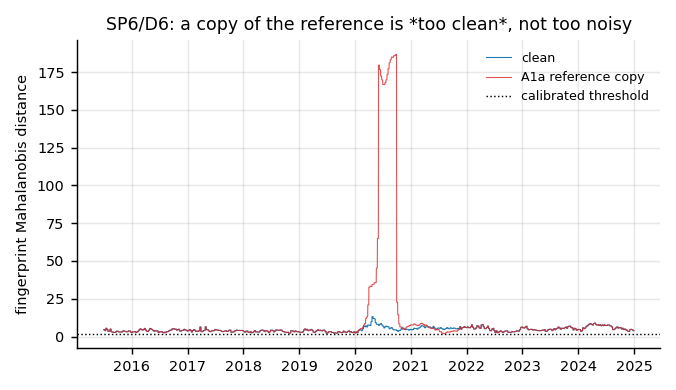
\includegraphics[width=0.98\linewidth,height=0.34\textheight,keepaspectratio]{figures/report_fig1.png}
\par\smallskip
\parbox{0.94\linewidth}{\small\itshape Figure 3 — spectral-\allowbreak{fingerprint example: the self-\allowbreak{}normalised distance moves when the sensor is replaced by a copy of the reference.}}
\end{center}


\begin{center}
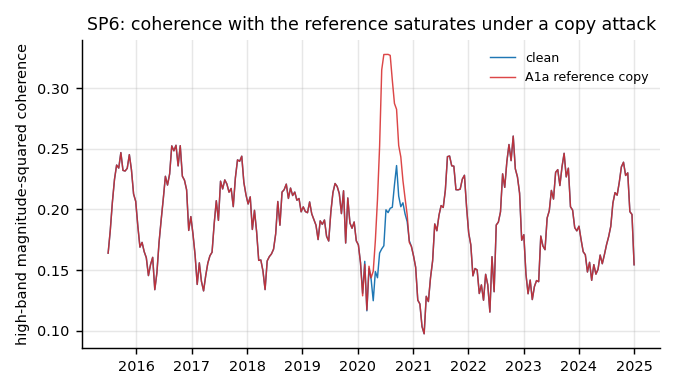
\includegraphics[width=0.98\linewidth,height=0.34\textheight,keepaspectratio]{figures/report_fig2.png}
\par\smallskip
\parbox{0.94\linewidth}{\small\itshape Figure 4 — sensor/\allowbreak{reference magnitude-\allowbreak{}squared coherence per band, honest versus attacked.}}
\end{center}

\end{document}
